\documentclass[aspectratio=169,11pt]{beamer}

\usetheme{Madrid}
\usecolortheme{default}
\usepackage{lmodern}
\usepackage[utf8]{inputenc}
\usepackage[T1]{fontenc}
\usepackage{amsmath,amssymb}
\usepackage{booktabs}
\usepackage{tikz}
\usetikzlibrary{arrows.meta, positioning}
\usepackage{listings}
\usepackage{xcolor}

\definecolor{manifold}{RGB}{30,90,170}
\setbeamercolor{structure}{fg=manifold}
\setbeamertemplate{navigation symbols}{}
\setbeamertemplate{footline}[frame number]

\title[MANIFOLD]{MANIFOLD}
\subtitle{A mathematical engine for mapping vulnerabilities}
\author{MANIFOLD Project}
\institute{Typed IR $\cdot$ geometry $\cdot$ topology $\cdot$ formal verification}
\date{2026}

\begin{document}

\begin{frame}
  \titlepage
\end{frame}

\begin{frame}{The problem: prioritize, don't detect}
  \begin{itemize}
    \item Classic SAST enumerates \emph{patterns}: the real bottleneck is not
          \emph{detecting} sinks but \emph{deciding which one to verify}.
    \item On OWASP Benchmark~1.2 the Youden index $J=\mathrm{TPR}-\mathrm{FPR}$ collapses:
          SonarQube $J\approx+0.01$, CodeQL $J\approx+0.22$.
    \item \textbf{Question:} can a scalar field $V(x)$ over the program graph
          prioritize the vulnerable sink?
  \end{itemize}
\end{frame}

\begin{frame}{Main experiment: the prioritization oracle}
  \begin{center}
  \small
  \begin{tabular}{lcccc}
  \toprule
  Ranking (902 vulnerable cases) & MRR & R@1 & NDCG@5 \\
  \midrule
  DFS (source order) & 0.848 & 0.755 & 0.882 \\
  raw taint & \textbf{0.894} & \textbf{0.847} & \textbf{0.916} \\
  fused $V(x)$ & 0.872 & 0.805 & 0.899 \\
  random & $0.688\pm0.056$ & 0.487 & 0.762 \\
  \bottomrule
  \end{tabular}
  \end{center}
  \vspace{1mm}
  \textbf{Per-signal AUC} (does it predict the vulnerable sink?):
  taint $0.895$ · formal $0.878$ · spectral $0.496$ ·
  topological $0.500$ · geometric $\mathbf{0.376}$.
\end{frame}

\begin{frame}{The honest result}
  \begin{itemize}
    \item $V(x)$ does \textbf{not} beat raw taint: it is slightly worse ($0.872$ vs.\ $0.894$).
    \item Spectral/topological: \emph{indistinguishable from chance}; curvature: \emph{worse than chance}.
    \item \textbf{Publishable (negative) finding:} on OWASP Benchmark the geometric
          and topological priors \emph{do not survive beyond taint}.
    \item $\Rightarrow$ MANIFOLD's value is in the \emph{formal} layer
          (verification), not the geometric prior. L1/L2/L5: \emph{not supported}.
  \end{itemize}
\end{frame}

\begin{frame}{The core idea}
  \begin{center}
  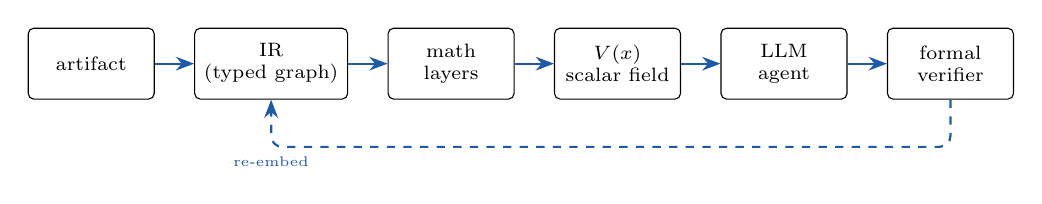
\begin{tikzpicture}[
    node distance=4mm and 5mm,
    box/.style={draw, rounded corners=2pt, minimum height=9mm, minimum width=16mm, align=center, font=\scriptsize},
    arr/.style={-{Stealth}, thick, color=manifold}
  ]
  \node[box] (art) {artifact};
  \node[box, right=of art] (ir) {IR\\(typed graph)};
  \node[box, right=of ir] (layers) {math\\layers};
  \node[box, right=of layers] (v) {$V(x)$\\scalar field};
  \node[box, right=of v] (agent) {LLM\\agent};
  \node[box, right=of agent] (verif) {formal\\verifier};
  \draw[arr] (art) -- (ir);
  \draw[arr] (ir) -- (layers);
  \draw[arr] (layers) -- (v);
  \draw[arr] (v) -- (agent);
  \draw[arr] (agent) -- (verif);
  \draw[arr, dashed, rounded corners] (verif.south) -- ++(0,-6mm) -| (ir.south)
    node[pos=0.5, below, font=\tiny]{re-embed};
  \end{tikzpicture}
  \end{center}
  \begin{itemize}
    \item A vulnerability is \emph{not} a pattern: it is the \emph{violation of a structural invariant}.
  \end{itemize}
\end{frame}

\begin{frame}{The unified IR}
  \textbf{Program graph} $G=(V,E,\tau_V,\tau_E,\omega)$:
  \begin{itemize}
    \item \textbf{Nodes}: module, function, statement, source, sink, \texttt{gate}, \dots
    \item \textbf{Typed edges}: \texttt{control}, \texttt{data}, \texttt{call}, \texttt{taint}, \texttt{trust}, \texttt{auth}
    \item JSON shared Python$\leftrightarrow$Rust; artifact-agnostic.
  \end{itemize}
  \vspace{2mm}
  \textbf{Multi-domain}: the \emph{same} IR is produced from
  \begin{itemize}
    \item Python / Java (tree-sitter), binaries (\texttt{objdump} or \texttt{angr}/\texttt{CFGFast}),
    \item OpenAPI (API surface), LLM agents (tool/trust graph).
  \end{itemize}
\end{frame}

\begin{frame}{Mathematical layers}
  \begin{columns}[T]
    \begin{column}{0.5\textwidth}
      \textbf{Spectral} ($L=D-A$)\\
      $\lambda_2$, Fiedler vector, embedding.
      \vspace{2mm}
      \textbf{Topological (TDA)}\\
      persistent homology $H_0,H_1$, Mapper.
      \vspace{2mm}
      \textbf{Geometric}\\
      Ollivier--Ricci / Forman--Ricci; Sinkhorn.
    \end{column}
    \begin{column}{0.5\textwidth}
      \textbf{Algebraic}\\
      taint lattice; naturality (categories).
      \vspace{2mm}
      \textbf{Formal}\\
      symbolic execution $+$ SMT (Z3); reachability.
      \vspace{2mm}
      \textbf{Directed}\\
      Chung Laplacian (SCC $+$ Perron).
    \end{column}
  \end{columns}
  \vspace{3mm}
  \begin{center}
  $V(x) = \sigma\!\big(\sum_i \alpha_i\, s_i(x)\big)$ \quad (calibrable weights $\alpha_i$)
  \end{center}
\end{frame}

\begin{frame}{Mapping laws (feature $\to$ vulnerability)}
  \begin{center}
  \begin{tabular}{cll}
  \toprule
  \# & Mathematical feature & Class \\
  \midrule
  L1 & curvature $\kappa \ll 0$ (chokepoint) & privilege escalation \\
  L2 & persistent $H_1$ generator & reentrancy / recursion \\
  L3 & Fiedler cut & injection across trust \\
  L4 & taint crossing an \texttt{auth} edge & naturality violation \\
  L5 & persistence outlier & real vs.\ spurious feature \\
  L6 & $\mathrm{SAT}(\phi_{\text{bad}})$ & concrete exploit \\
  \bottomrule
  \end{tabular}
  \end{center}
\end{frame}

\begin{frame}[fragile]{The neuro-symbolic agent}
  \begin{enumerate}
    \item \textbf{Map}: IR $+$ signals $V(x)$, persistence, curvature.
    \item \textbf{Hypothesize}: the LLM proposes over prioritized regions.
    \item \textbf{Verify}: Z3 / taint / topology proves or refutes.
    \item \textbf{Refine} and \textbf{report} (concrete witness).
  \end{enumerate}
  \vspace{2mm}
  Division of labor: mathematics proposes \emph{regions}; the LLM proposes
  \emph{hypotheses}; the solver proposes \emph{proofs}. \\[1mm]
  \textbf{Verification grammar}: structured spec
  \texttt{(sink, source, line, category)} --- the LLM never emits SMT-LIB.
\end{frame}

\begin{frame}{Results: OWASP Benchmark 1.2}
  \begin{center}
  \small
  \begin{tabular}{lcccccc}
  \toprule
  \textbf{Tool} & \textbf{TPR} & \textbf{FPR} & \textbf{Prec.} & \textbf{F1} & \textbf{J} & \textbf{Time} \\
  \midrule
  SonarQube\textsuperscript{(a)} & 0.956 & 0.946 & 0.330 & 0.490 & +0.010 & \textasciitilde3 min \\
  CodeQL\textsuperscript{(a)} & 0.902 & 0.682 & 0.603 & 0.744 & +0.220 & \textasciitilde18 min \\
  \textbf{MANIFOLD} adapter\textsuperscript{(b)} & 0.842 & 0.674 & 0.572 & 0.681 & \textbf{+0.168} & \textasciitilde45 s \\
  MANIFOLD adapter $+$ Z3\textsuperscript{(b)} & 0.834 & 0.776 & 0.549 & 0.662 & +0.057 & \textasciitilde4 min \\
  \bottomrule
  \end{tabular}
  \end{center}

  \vspace{1mm}
  {\footnotesize (a) reported in public evaluations. (b) \textbf{measured} (Z3 adds witnesses, not precision).}
\end{frame}

\begin{frame}{Ablation: where the gain comes from}
  \begin{center}
  \small
  \begin{tabular}{lccc}
  \toprule
  Variant (taint categories) & Prec. & Recall & F1 \\
  \midrule
  Initial naive adapter & 0.515 & 0.426 & 0.466 \\
  $+$ branch-join, receiver/state taint, sink coverage & 0.530 & 0.856 & 0.655 \\
  $+$ XSS response-writer restriction (final) & \textbf{0.549} & \textbf{0.834} & \textbf{0.662} \\
  \midrule
  final, without branch-join & 0.515 & 0.555 & 0.535 \\
  \bottomrule
  \end{tabular}
  \end{center}
  \begin{itemize}
    \item \textbf{Branch-join} (lattice join) is the \emph{recall} lever ($+0.28$).
    \item The \textbf{HTTP response-writer restriction} is the \emph{precision} lever.
    \item Residual errors are adversarial cases --- what $V(x)+$Z3 must recover.
  \end{itemize}
\end{frame}

\begin{frame}{Visualization and demo}
  \begin{itemize}
    \item \textbf{Manifold map}: IR graph with a force-directed layout; nodes by kind,
          edges by kind (red taint), purple \texttt{gate}.
    \item \textbf{Findings panel}: \emph{confirmed} (Z3 with witness) vs \emph{candidate}.
    \item \textbf{Self-contained HTML} (no dependencies) $+$ end-to-end demo on 10 artifacts.
  \end{itemize}
  \vspace{2mm}
  \begin{center}
  \texttt{python -m manifold.cli target --agent --viz out.html}
  \end{center}
\end{frame}

\begin{frame}{Conclusions and future work}
  \textbf{Conclusions}
  \begin{itemize}
    \item A typed IR fuses independent signals into a navigable field $V(x)$.
    \item The neuro-symbolic split (math/LLM/SMT) is the right one.
    \item On OWASP Benchmark: $F_1$ $0.466 \to 0.662$ with generic taint fixes alone.
  \end{itemize}
  \vspace{2mm}
  \textbf{Future work}
  \begin{itemize}
    \item Z3 verification for Java (closing the projected row).
    \item Directed homology and Sinkhorn at scale; calibrating $\alpha_i$ on real corpora.
    \item ELF/PE benchmarks (SARD) on the dual binary backend.
  \end{itemize}
\end{frame}

\begin{frame}
  \centering
  \Large\color{manifold}\textbf{Thank you}\\[4mm]
  \normalsize\color{black}
  MAP the code as a space; let geometry reveal the flaw.
\end{frame}

\end{document}
